\section*{Appendix}
\markboth{APPENDIX}{APPENDIX}
\addcontentsline{toc}{chapter}{Appendix}

\bigbreak

\subsection*{A. Input trajectories parsing algorithm}
\addcontentsline{toc}{section}{A. Input trajectories parsing algorithm}
\lstset{style=code-style-java}
\lstinputlisting[caption={Input trajectories parsing algorithm}, label={lst:parse-traj}] {listings/parsing.java}

\bigbreak

\subsection*{B. Polynomial Regression initiation}
\addcontentsline{toc}{section}{B. Polynomial Regression initiation}
\lstinputlisting[caption={Polynomial Regression initiation}, label={lst:pol-regr}] {listings/polRegr.java}

\bigbreak

\subsection*{C. Agglomerative Hierarchical Clustering}
\addcontentsline{toc}{section}{C. Agglomerative Hierarchical Clustering}
\lstinputlisting[caption={Clustering implementation}, label={lst:clust-impl}] {listings/clustImpl.java}

\bigbreak

\subsection*{D. Visualization of clustering results for static $\varepsilon$}
\addcontentsline{toc}{section}{D. Visualization of clustering results for static $\varepsilon$}
\begin{figure}[!htb]
	\centering
	\begin{subfigure}[!htb]{0.495\textwidth}
		\centering{}
		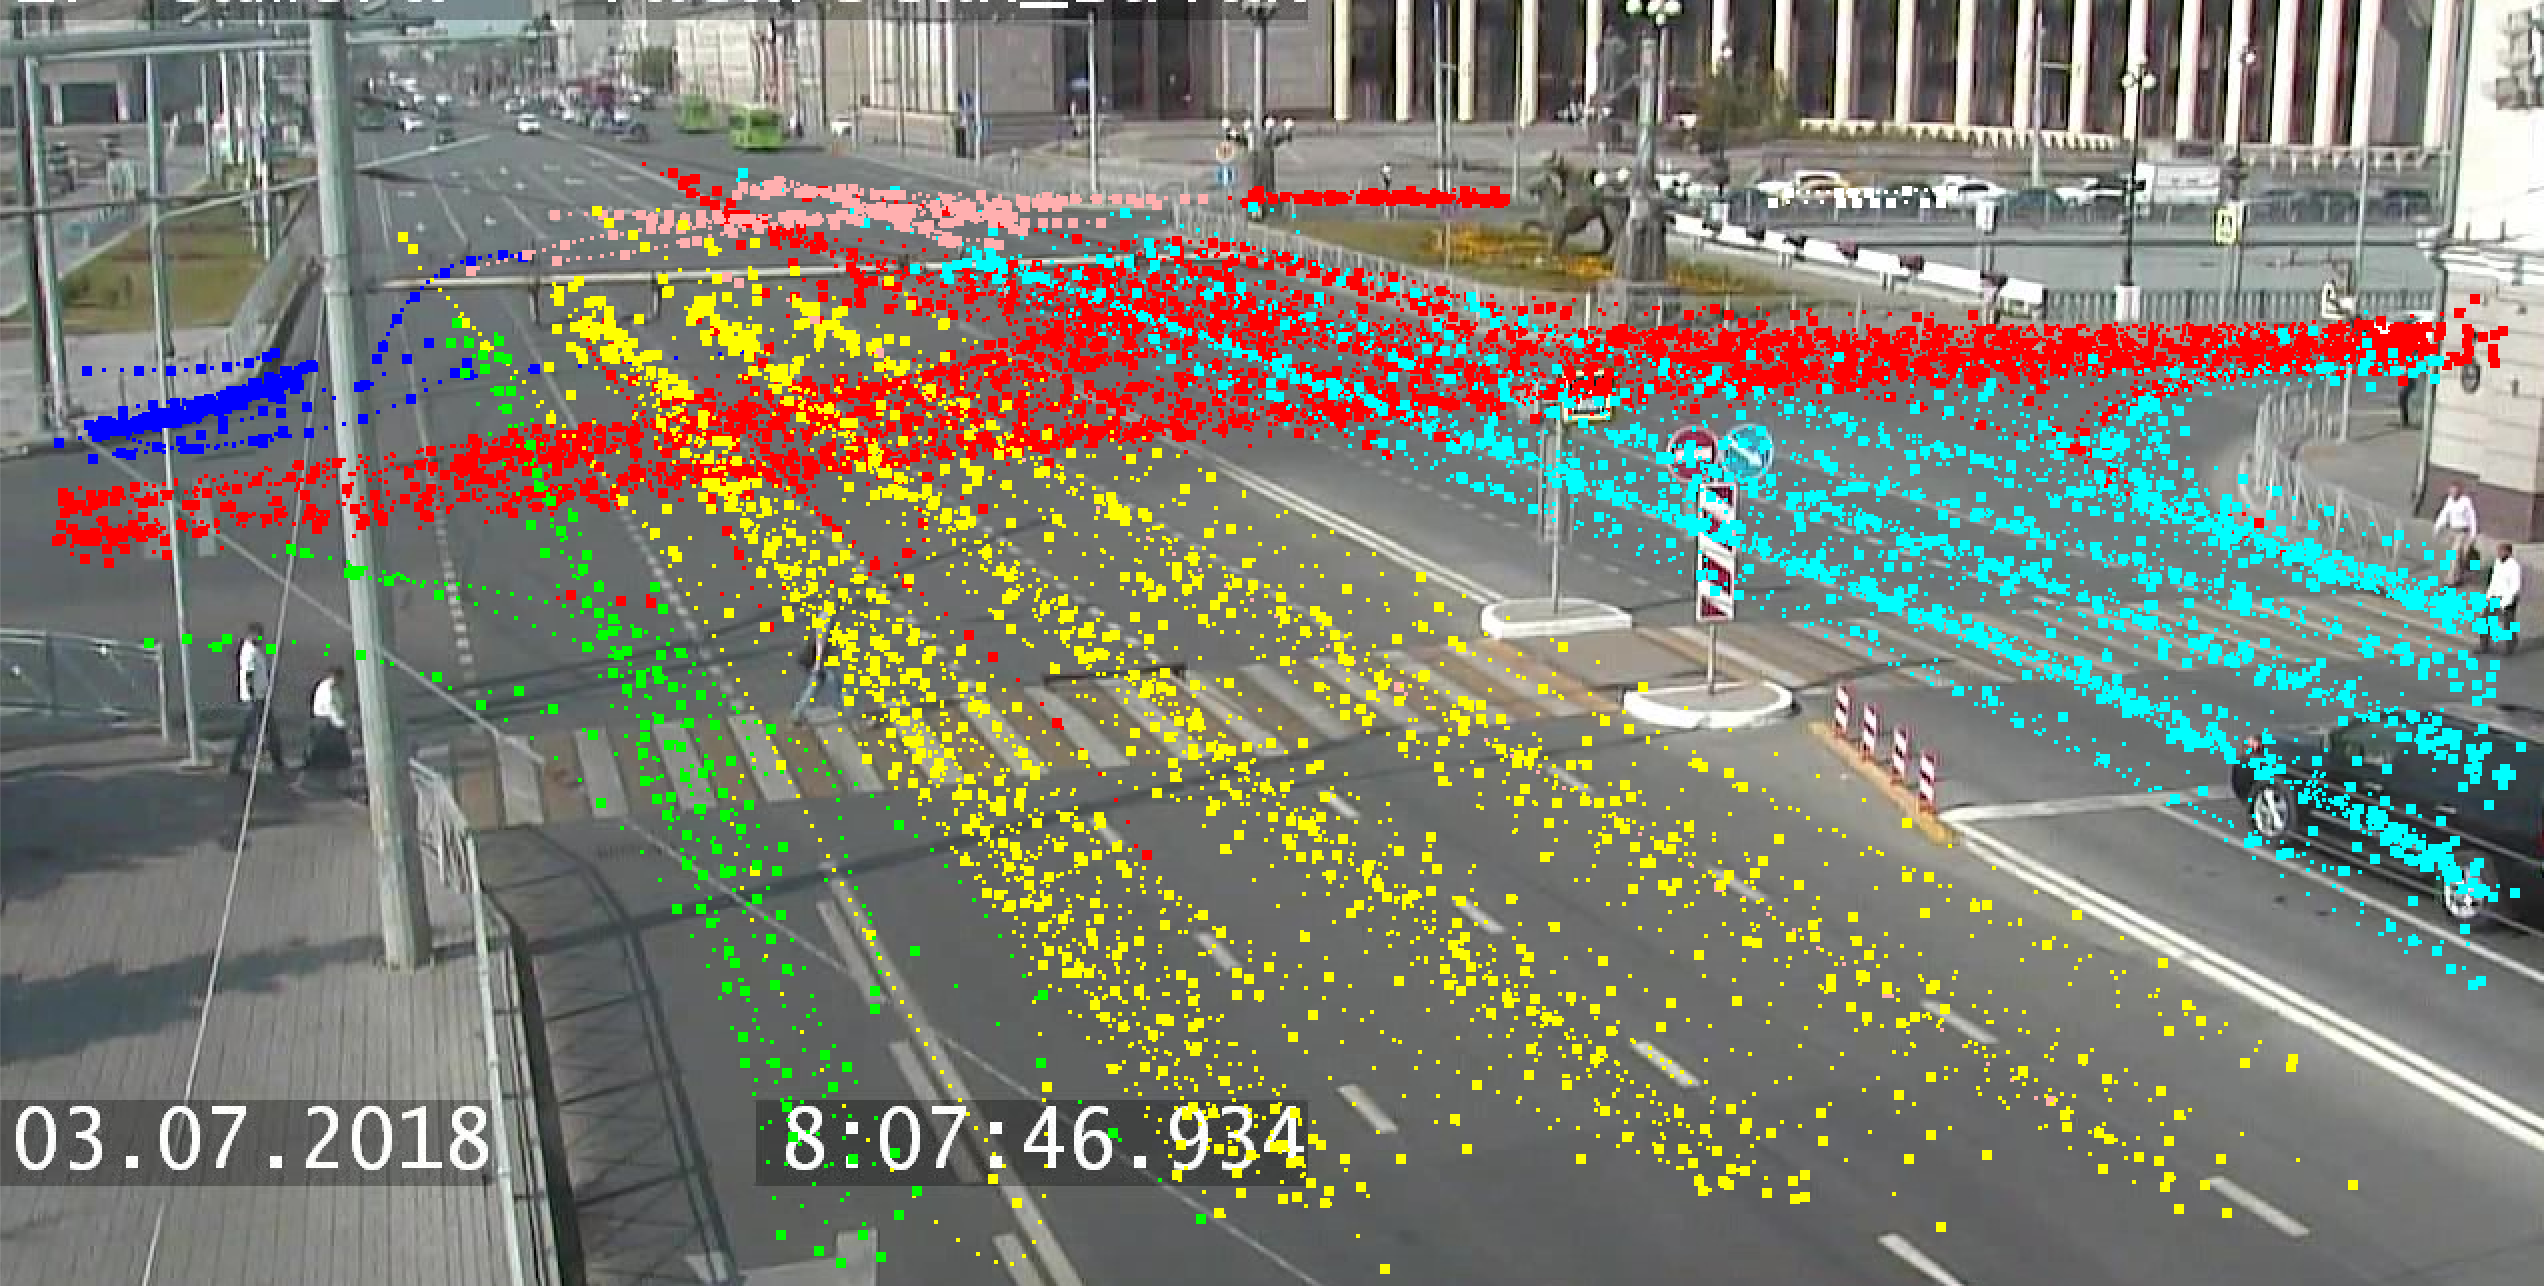
\includegraphics[width=\textwidth]{images/cl-res/1-7cl-01.png}
		\caption{7 clusters, DI = 0.88}
		\label{fig:1-7cl-01}
	\end{subfigure}
	\hfill
	\begin{subfigure}[!htb]{0.495\textwidth}
		\centering{}
		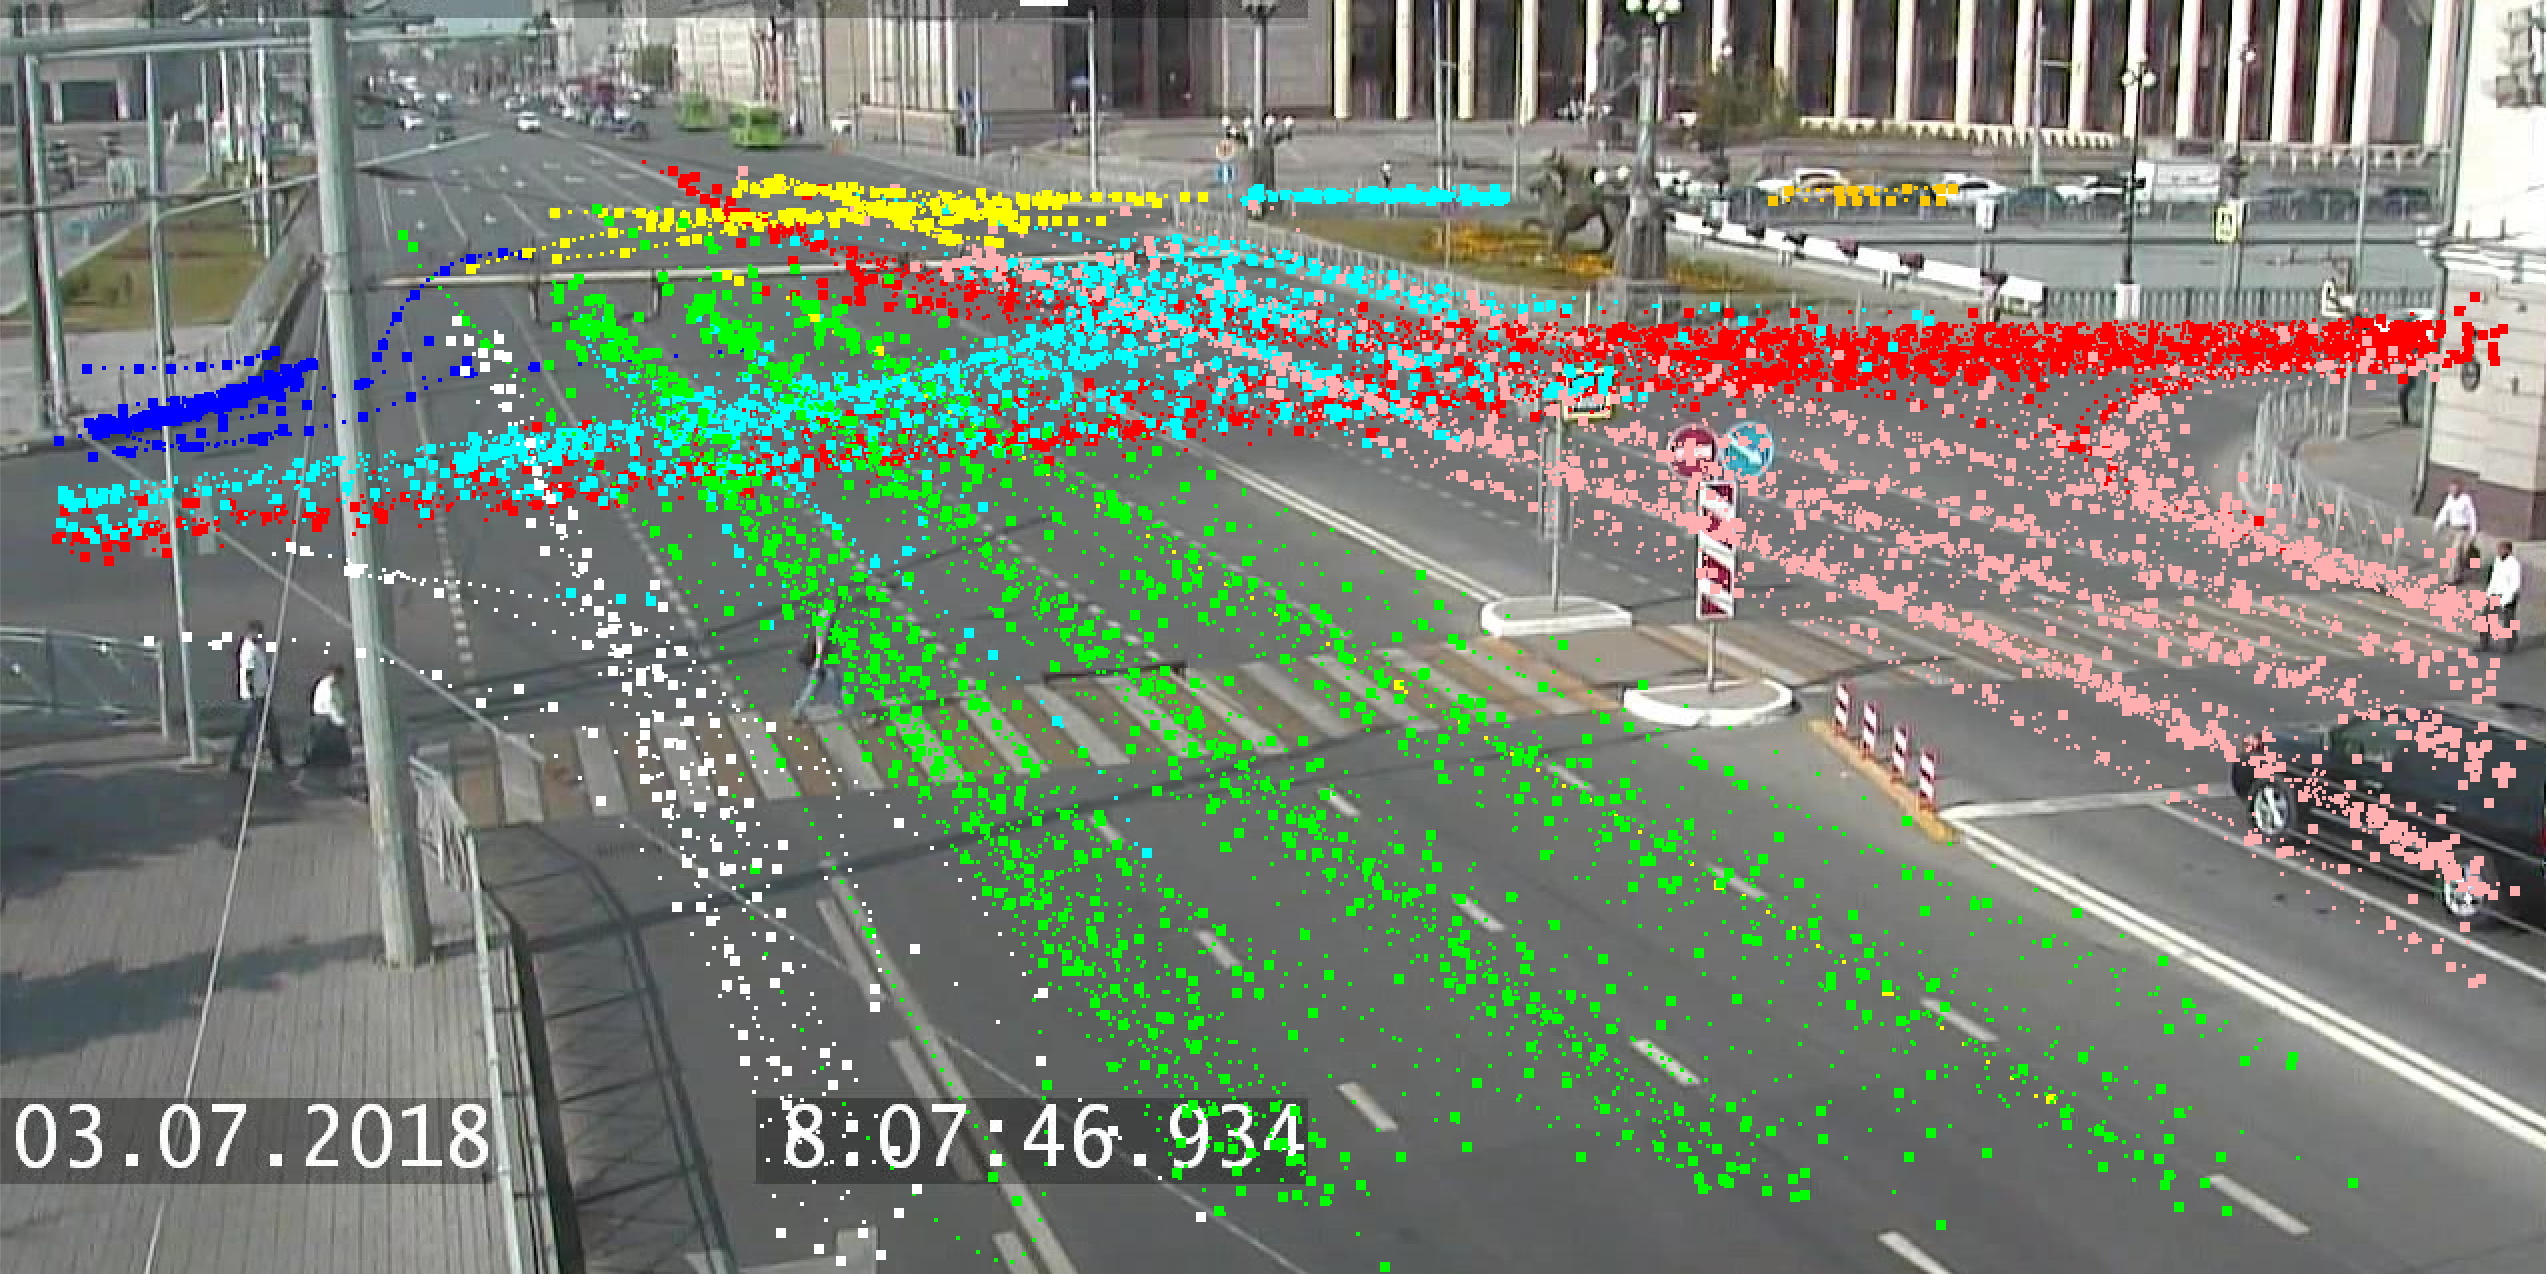
\includegraphics[width=\textwidth]{images/cl-res/1-8cl-01.png}
		\caption{8 clusters, DI = 0.83}
		\label{fig:1-8cl-01}
	\end{subfigure}
	\hfill
	\begin{subfigure}[!htb]{0.495\textwidth}
		\centering{}
		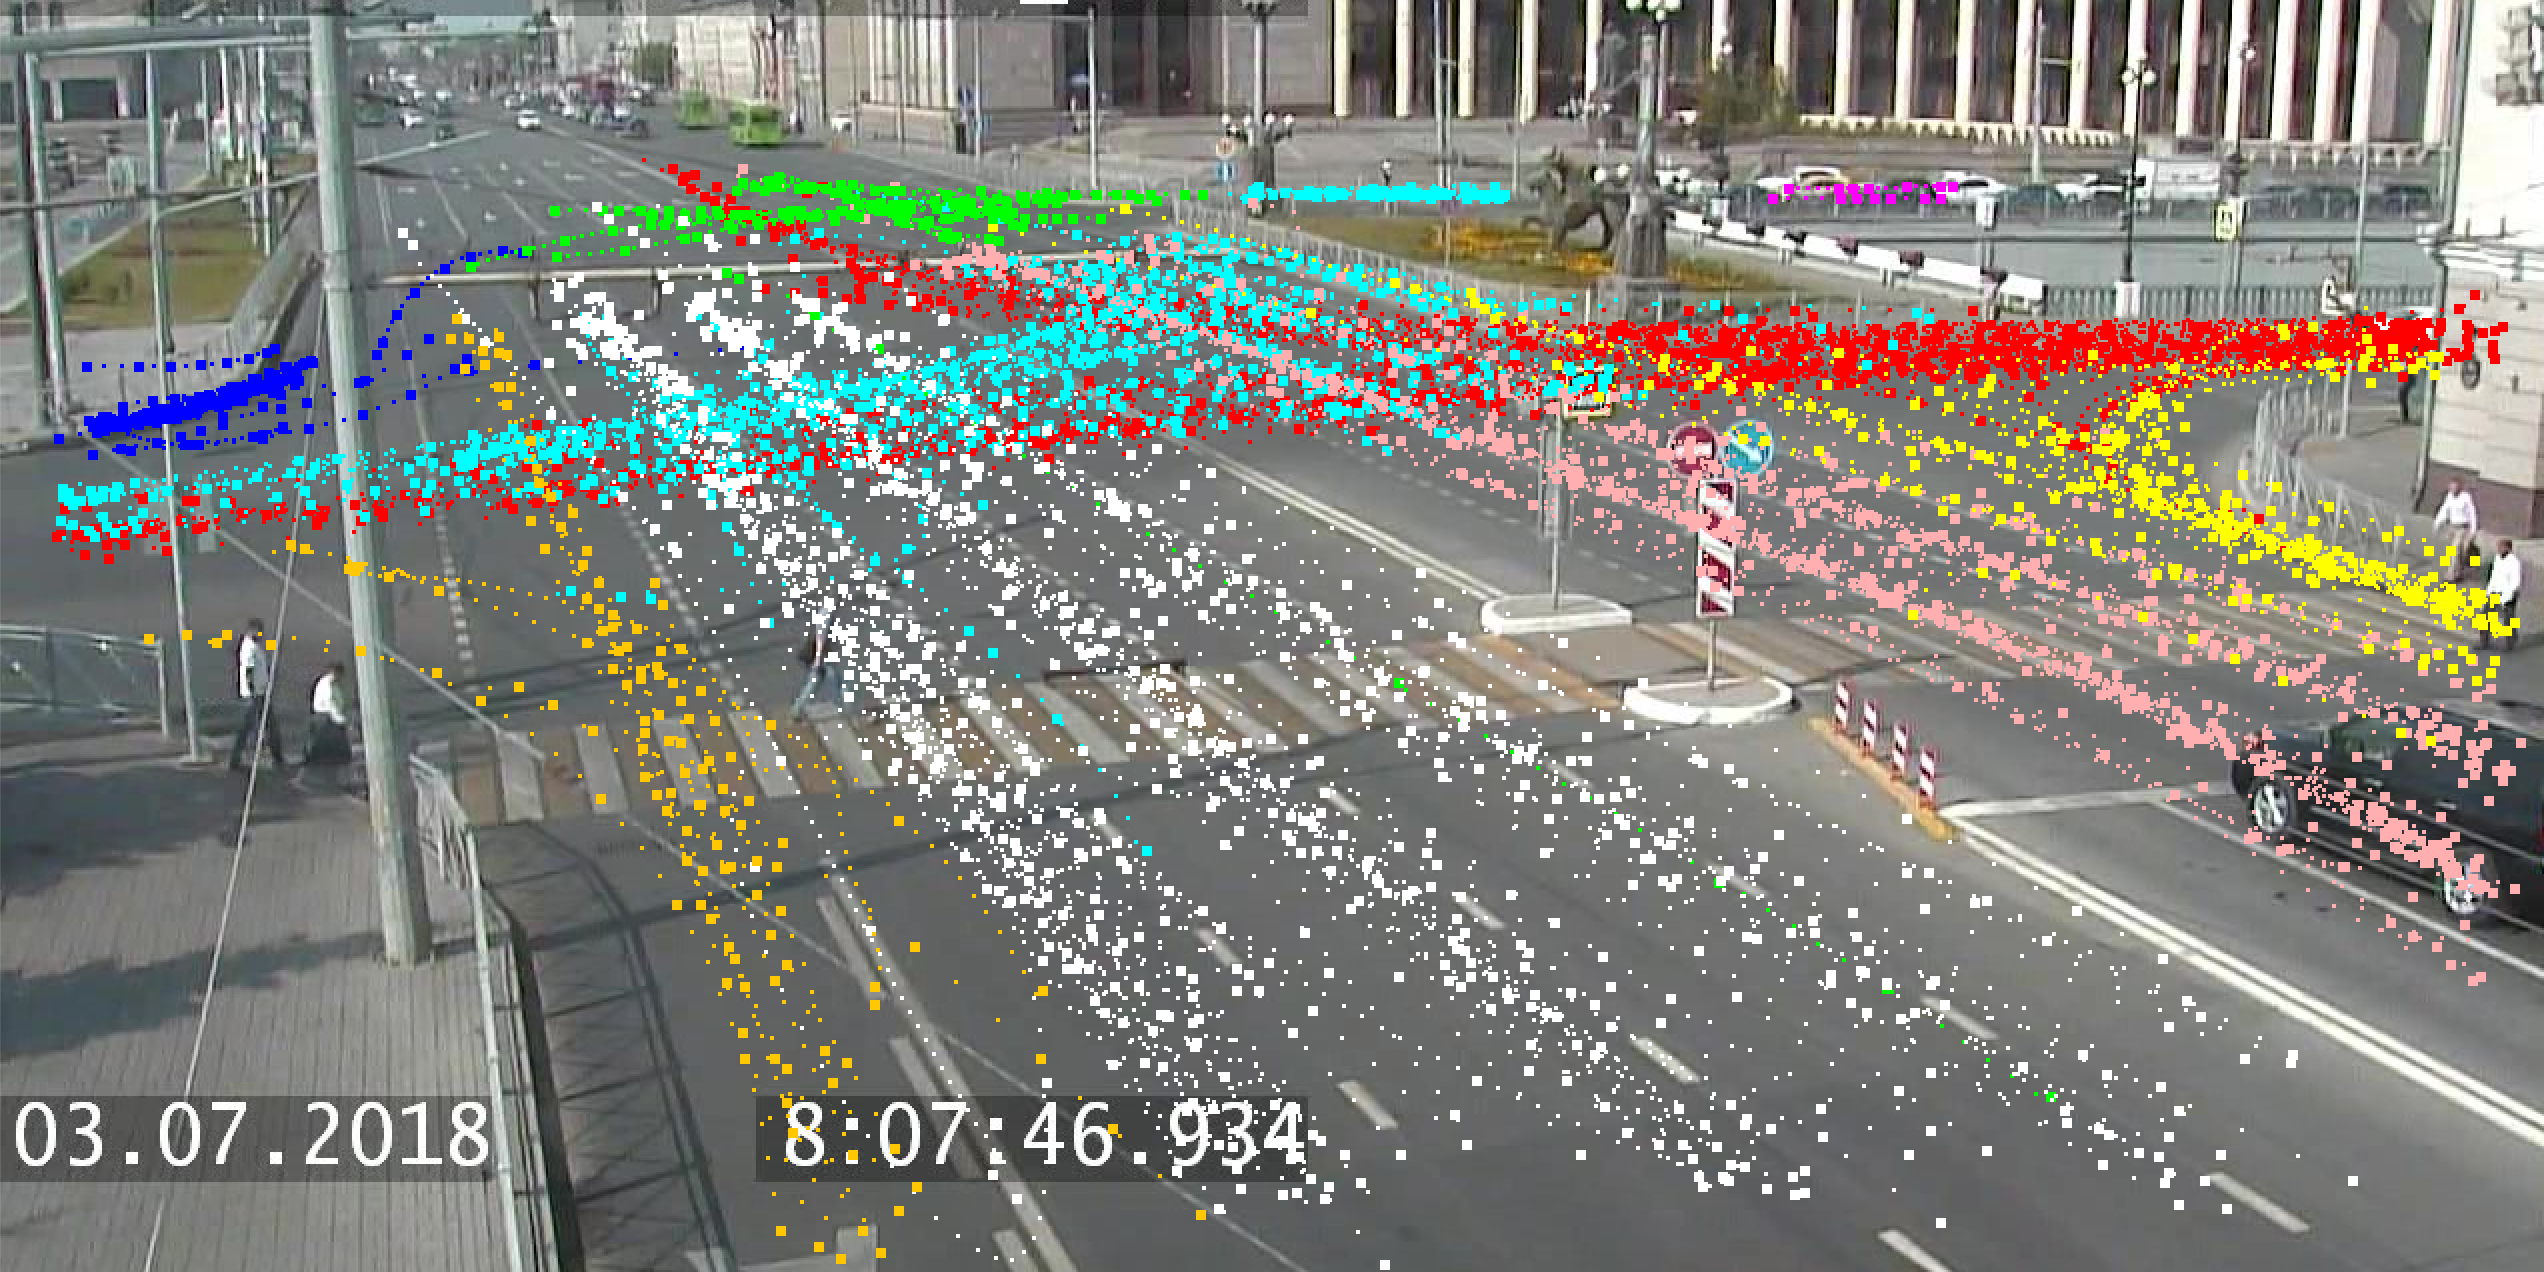
\includegraphics[width=\textwidth]{images/cl-res/1-9cl-01.png}
		\caption{9 clusters, DI = 0.77}
		\label{fig:1-9cl-01}
	\end{subfigure}
	\caption{Clustering results for static $\bm{\varepsilon}$, $coeff_\varepsilon = 0.1$ ($1.txt$)}
	\label{fig:clust-res-1-01}
\end{figure}

\begin{figure}[!htb]
	\centering
	\begin{subfigure}[!htb]{0.495\textwidth}
		\centering{}
		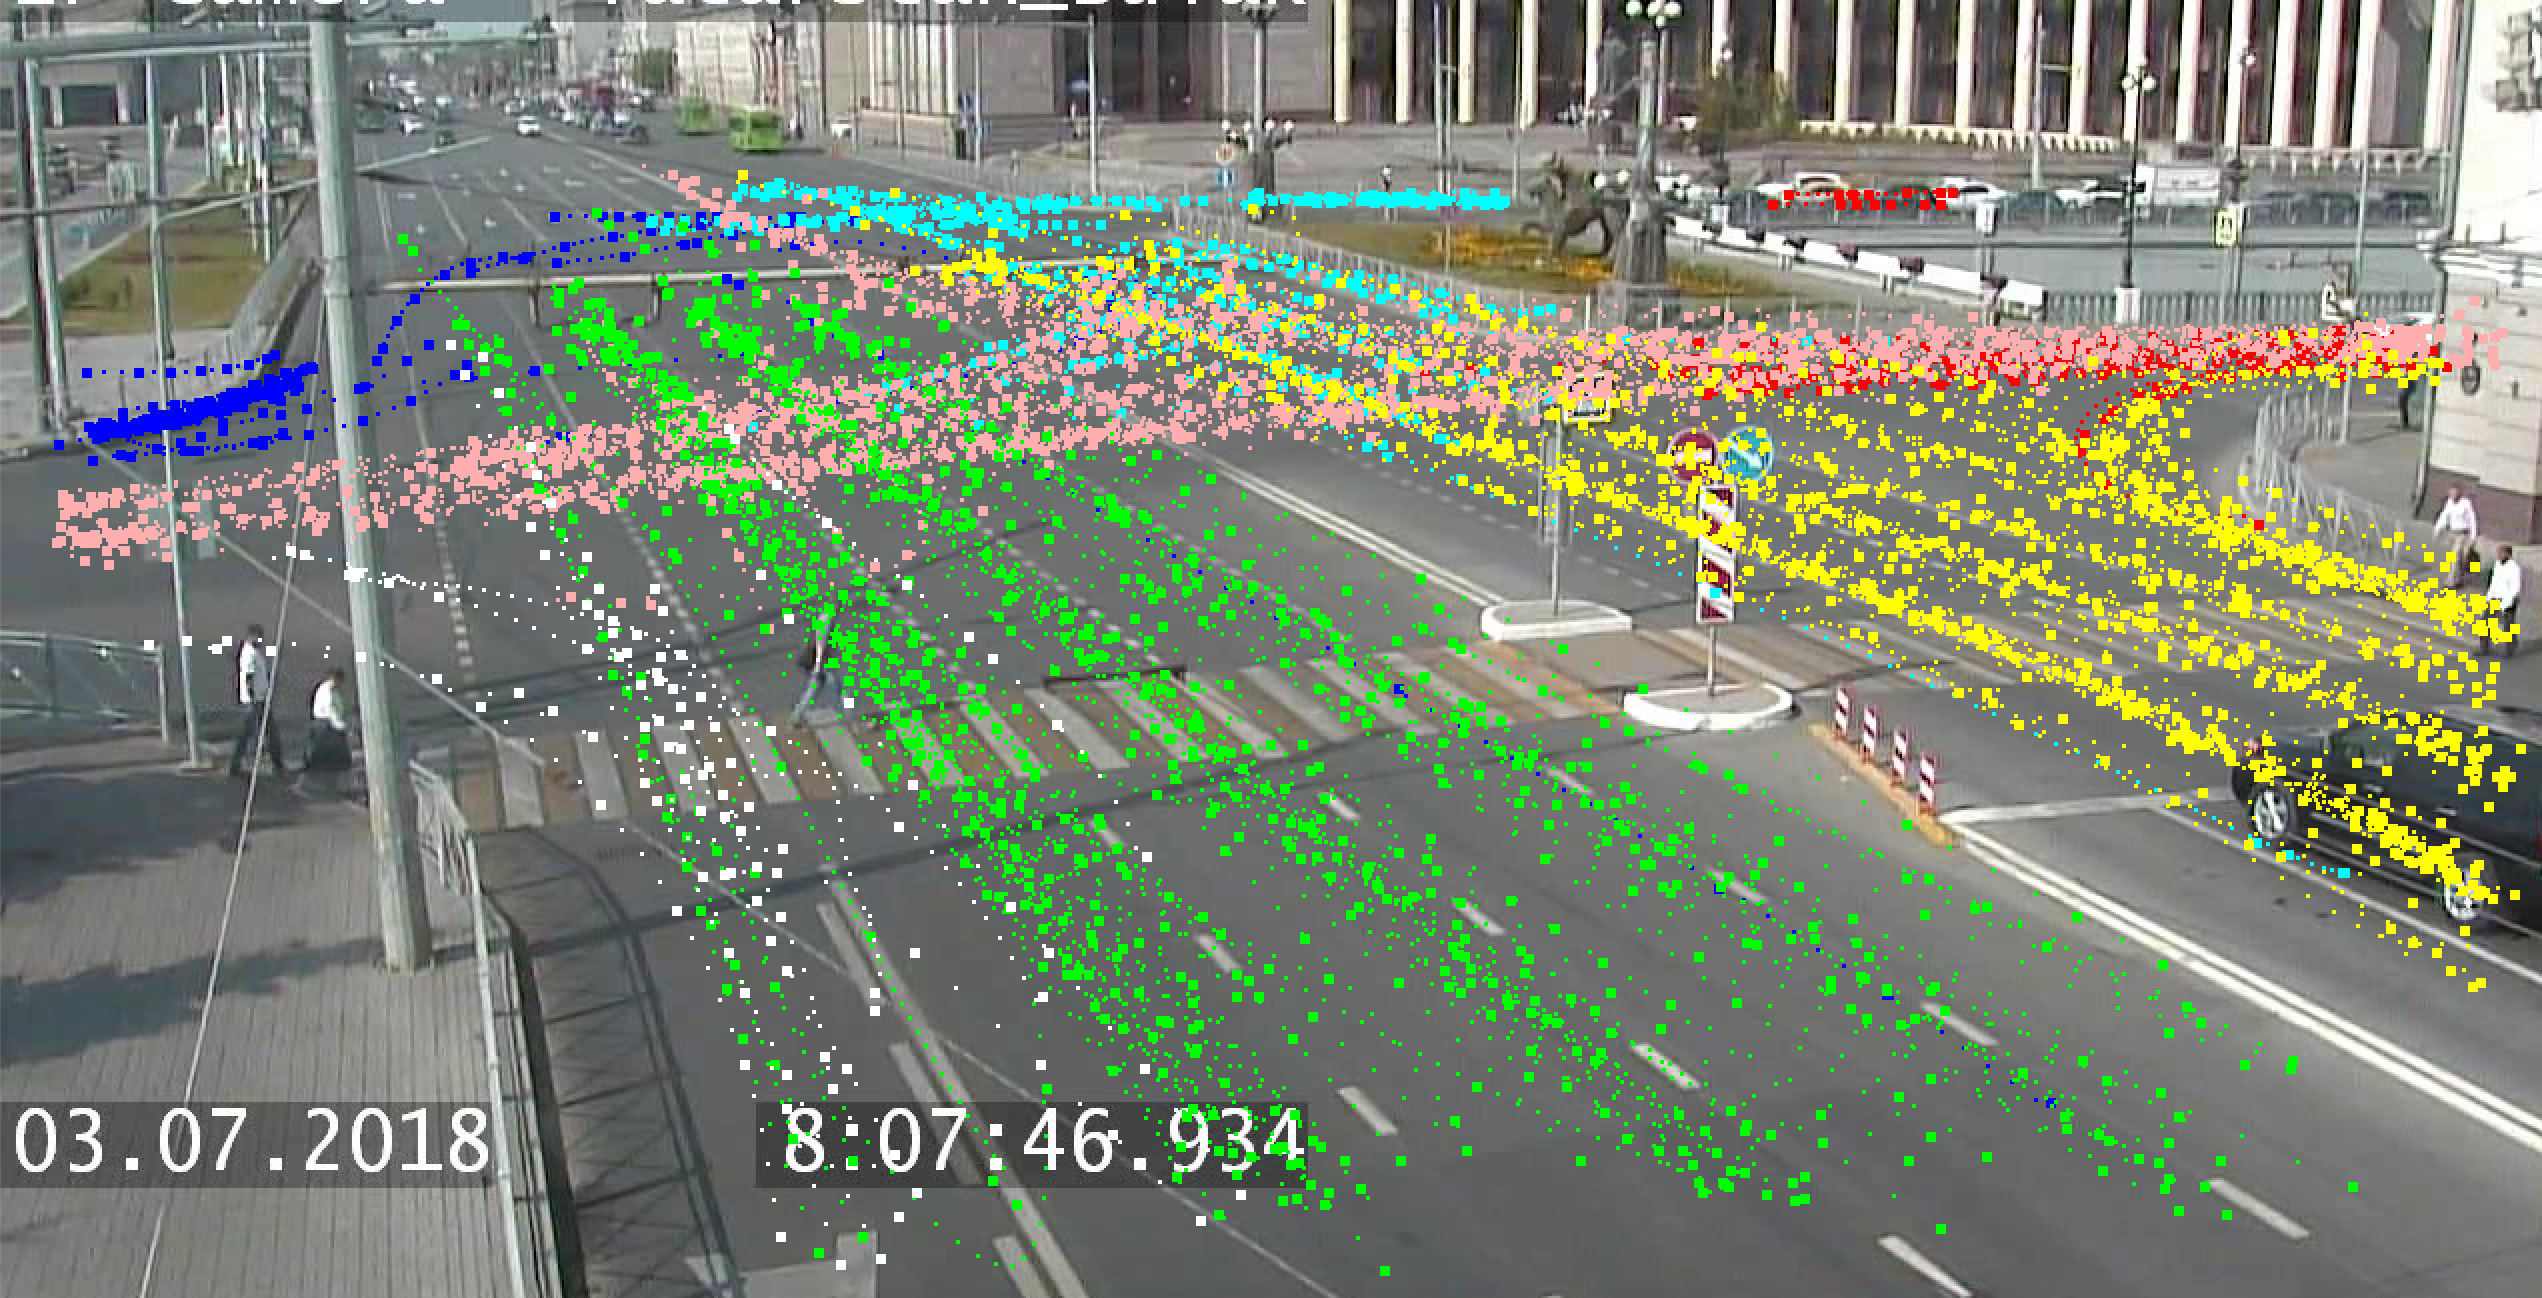
\includegraphics[width=\textwidth]{images/cl-res/1-7cl-015.png}
		\caption{7 clusters, DI = 0.68}
		\label{fig:1-7cl-015}
	\end{subfigure}
	\hfill
	\begin{subfigure}[!htb]{0.495\textwidth}
		\centering{}
		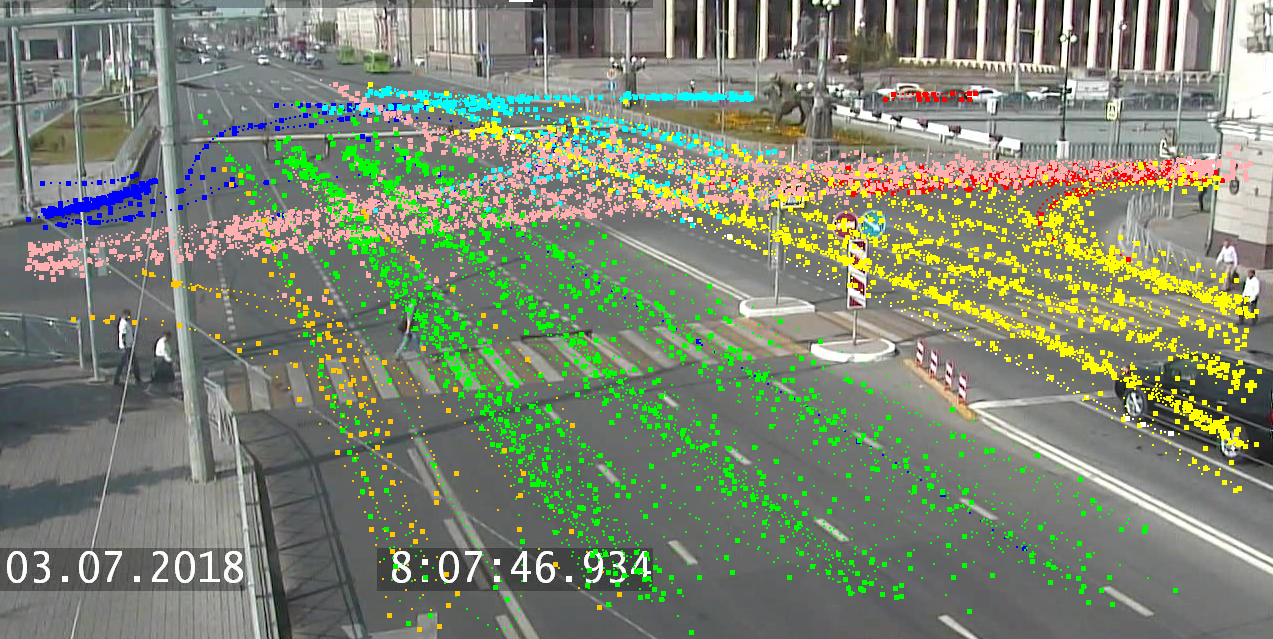
\includegraphics[width=\textwidth]{images/cl-res/1-8cl-015.png}
		\caption{8 clusters, DI = 0.63}
		\label{fig:1-8cl-015}
	\end{subfigure}
	\hfill
	\begin{subfigure}[!htb]{0.495\textwidth}
		\centering{}
		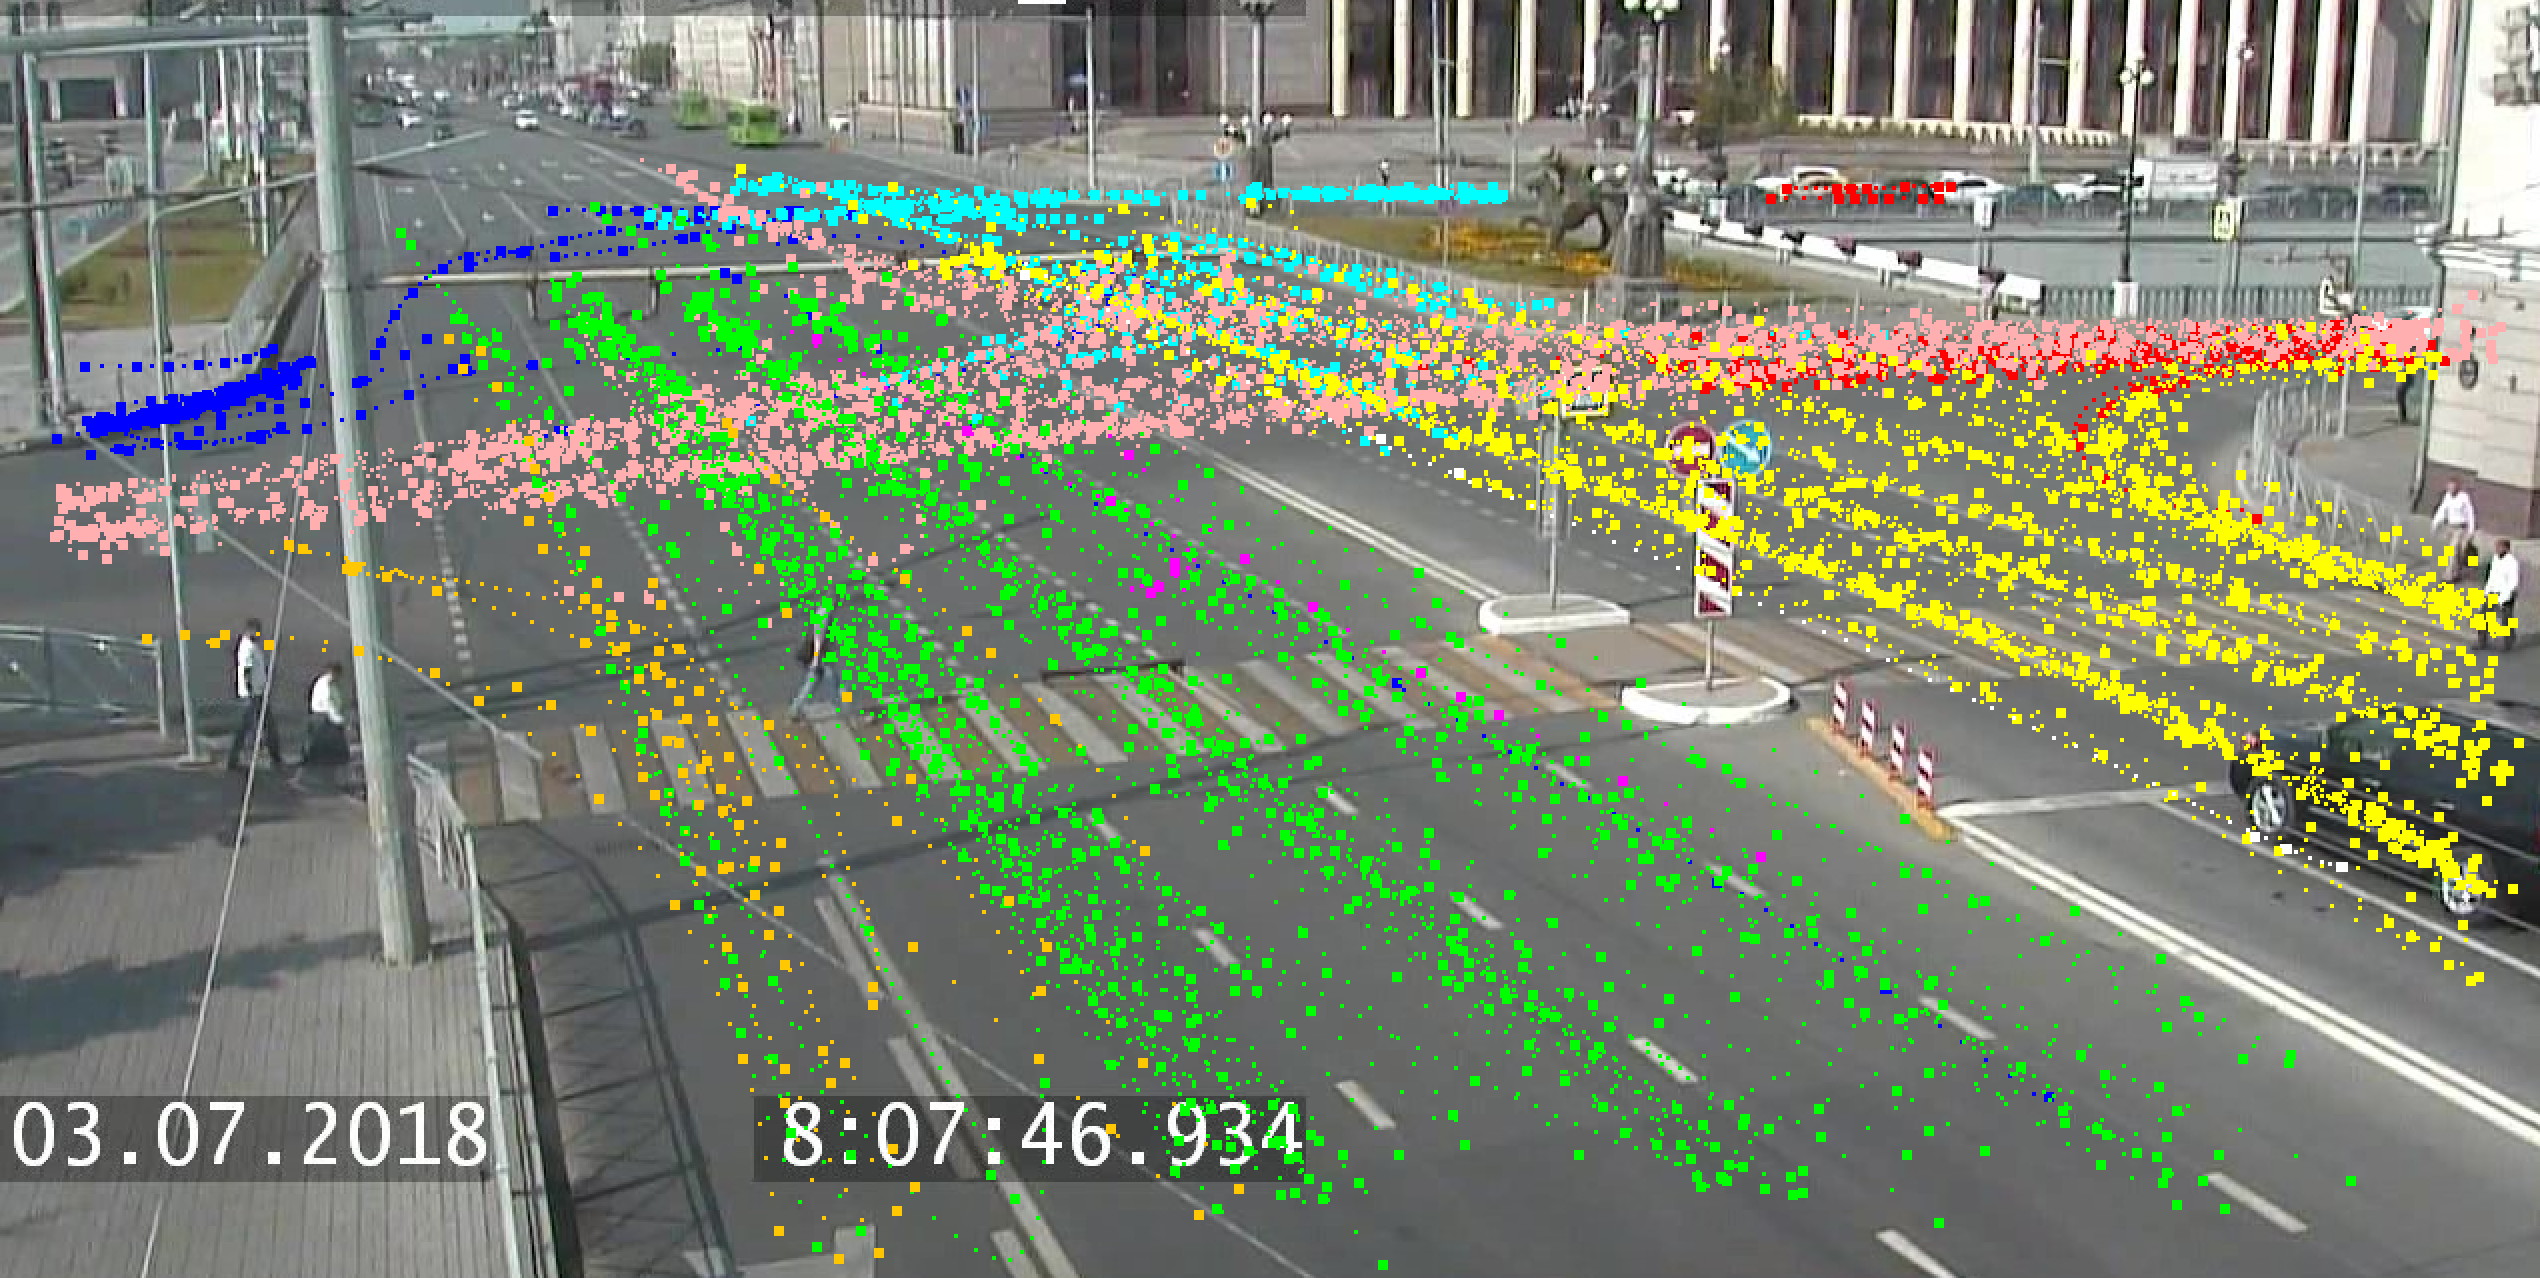
\includegraphics[width=\textwidth]{images/cl-res/1-9cl-015.png}
		\caption{9 clusters, DI = 0.62}
		\label{fig:1-9cl-015}
	\end{subfigure}
	\caption{Clustering results for static $\bm{\varepsilon}$, $coeff_\varepsilon = 0.15$ ($1.txt$)}
	\label{fig:clust-res-1-015}
\end{figure}

\begin{figure}[!htb]
	\centering
	\begin{subfigure}[!htb]{0.495\textwidth}
		\centering{}
		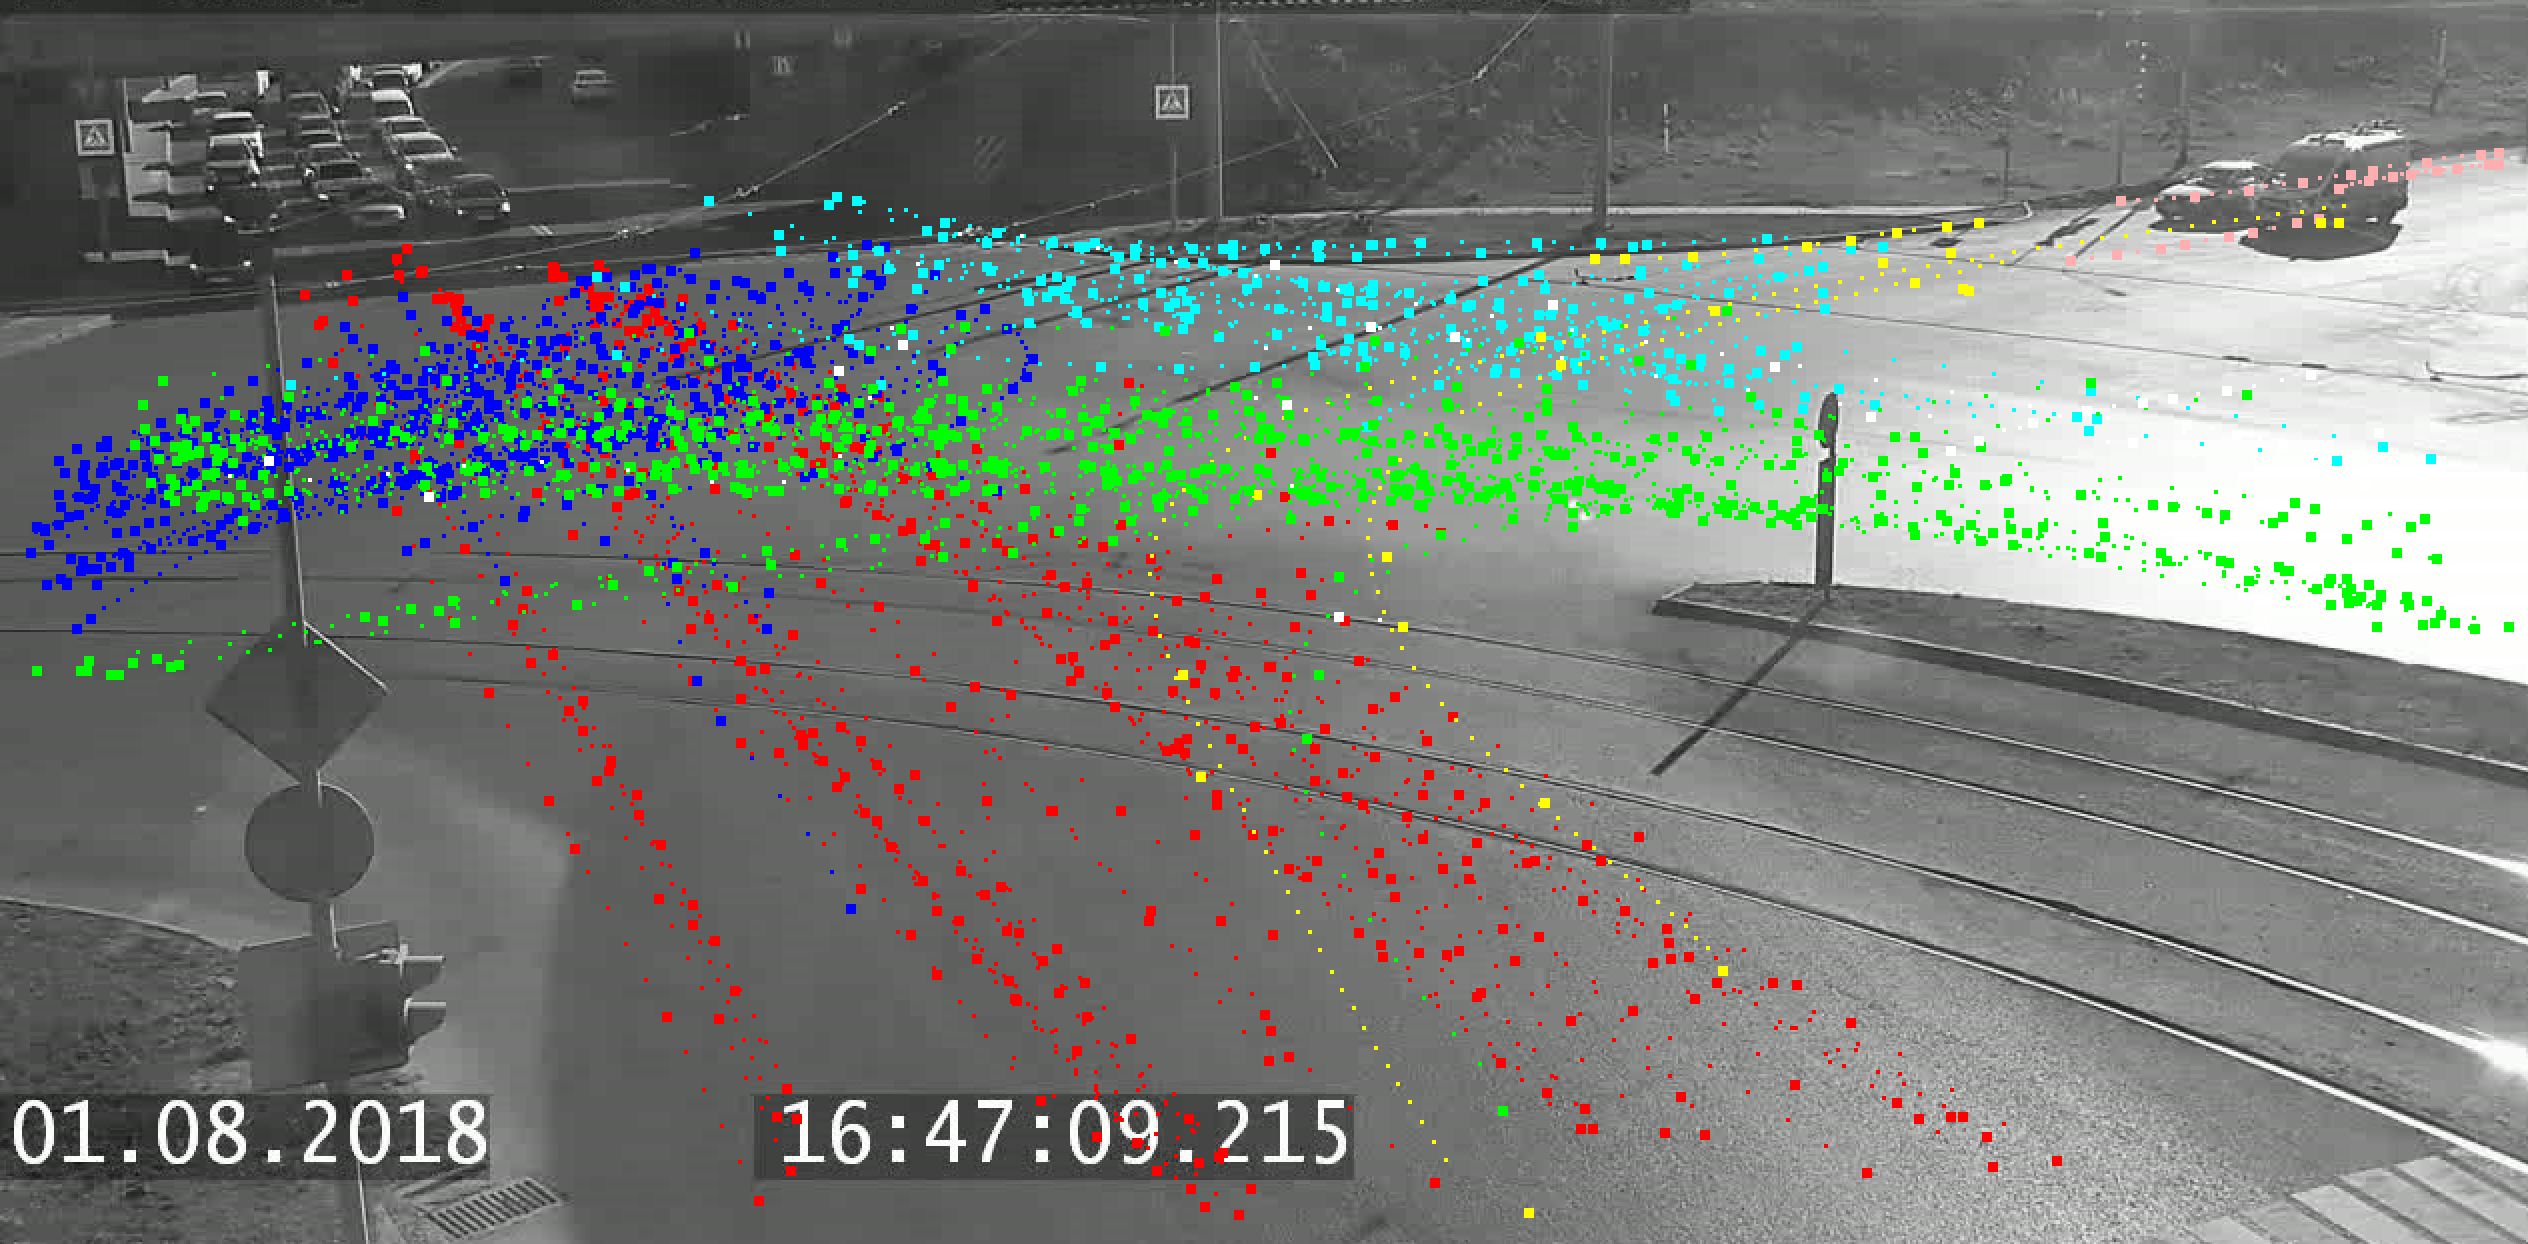
\includegraphics[width=\textwidth]{images/cl-res/2-7cl-01.png}
		\caption{7 clusters, DI = 0.80}
		\label{fig:2-7cl-01}
	\end{subfigure}
	\hfill
	\begin{subfigure}[!htb]{0.495\textwidth}
		\centering{}
		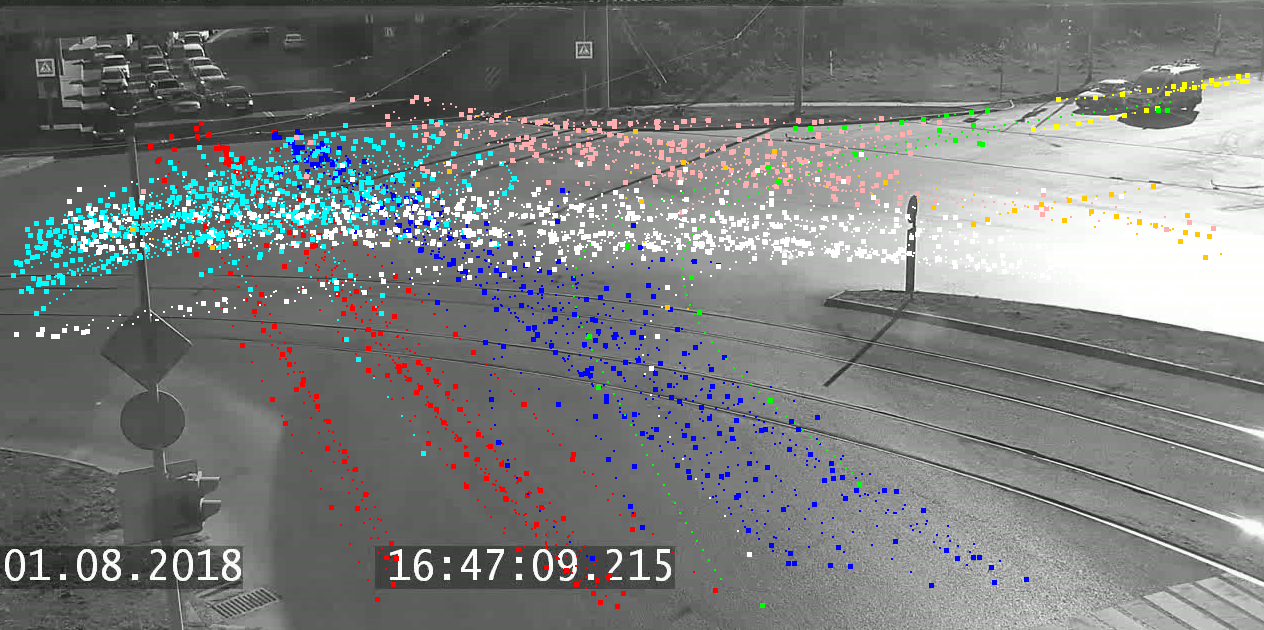
\includegraphics[width=\textwidth]{images/cl-res/2-8cl-01.png}
		\caption{8 clusters, DI = 0.80}
		\label{fig:2-8cl-01}
	\end{subfigure}
	\hfill
	\begin{subfigure}[!htb]{0.495\textwidth}
		\centering{}
		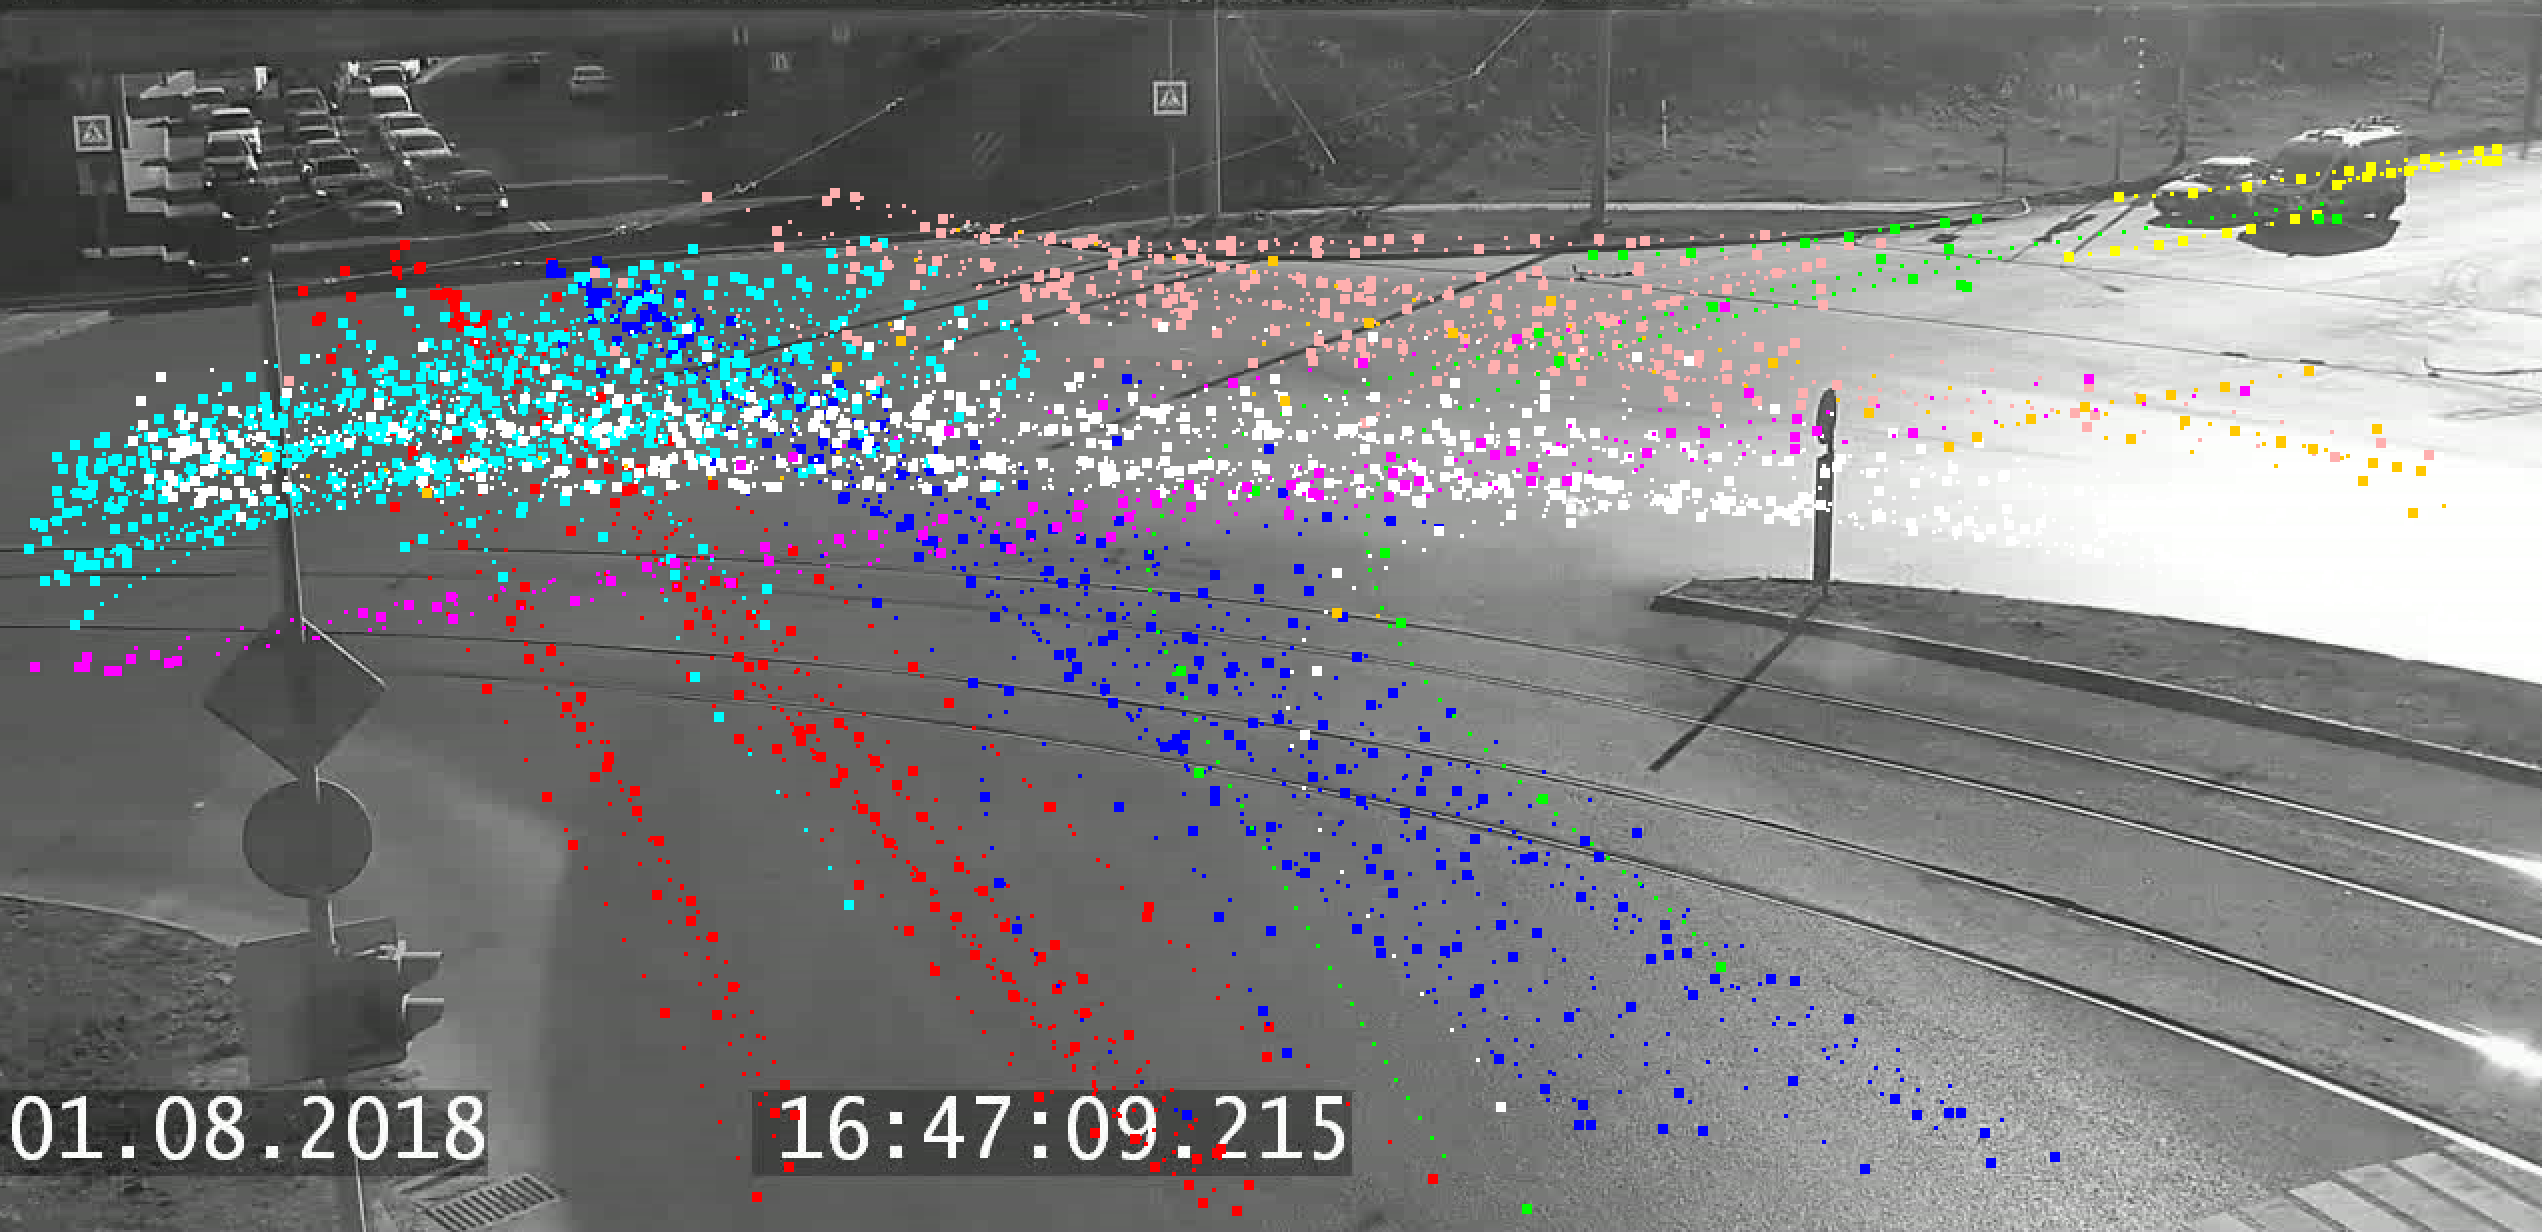
\includegraphics[width=\textwidth]{images/cl-res/2-9cl-01.png}
		\caption{9 clusters, DI = 0.78}
		\label{fig:2-9cl-01}
	\end{subfigure}
	\caption{Clustering results for static $\bm{\varepsilon}$, $coeff_\varepsilon = 0.1$ ($2.txt$)}
	\label{fig:clust-res-2-01}
\end{figure}

\begin{figure}[!htb]
	\centering
	\begin{subfigure}[!htb]{0.495\textwidth}
		\centering{}
		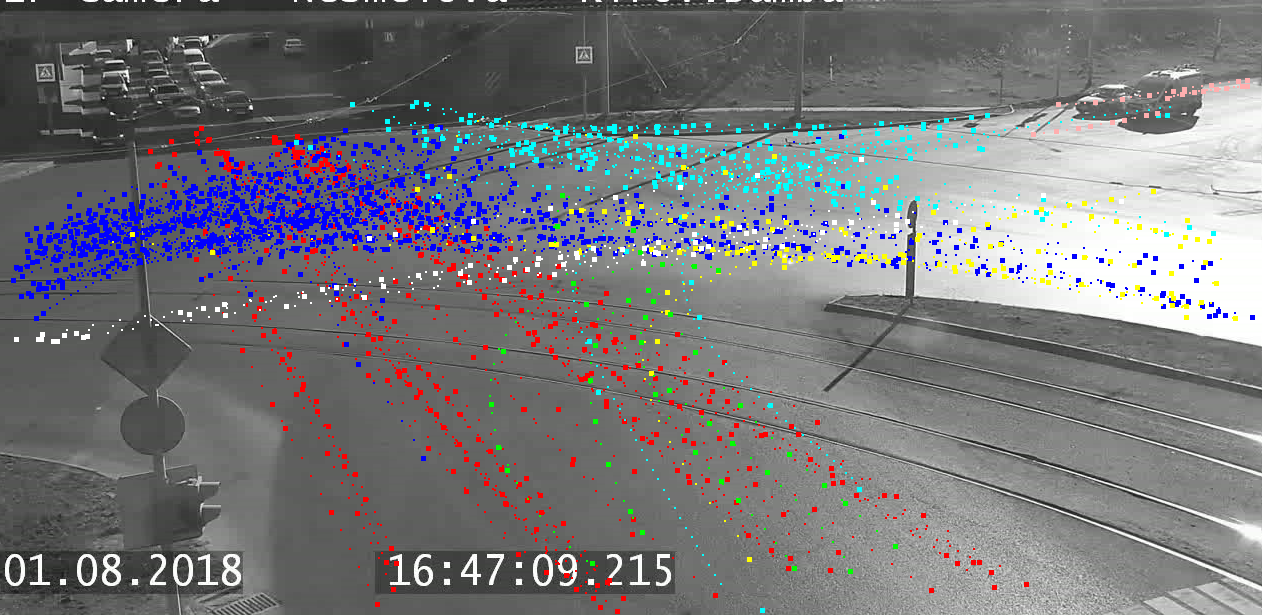
\includegraphics[width=\textwidth]{images/cl-res/2-7cl-015.png}
		\caption{7 clusters, DI = 0.67}
		\label{fig:2-7cl-015}
	\end{subfigure}
	\hfill
	\begin{subfigure}[!htb]{0.495\textwidth}
		\centering{}
		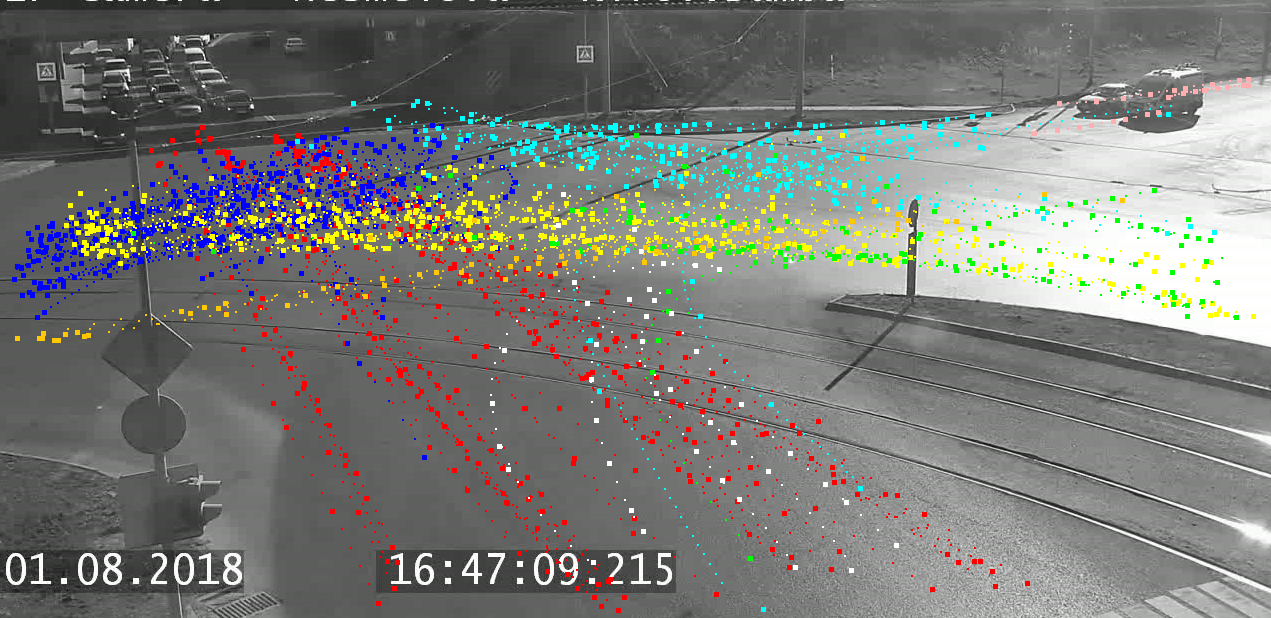
\includegraphics[width=\textwidth]{images/cl-res/2-8cl-015.png}
		\caption{8 clusters, DI = 0.64}
		\label{fig:2-8cl-015}
	\end{subfigure}
	\hfill
	\begin{subfigure}[!htb]{0.495\textwidth}
		\centering{}
		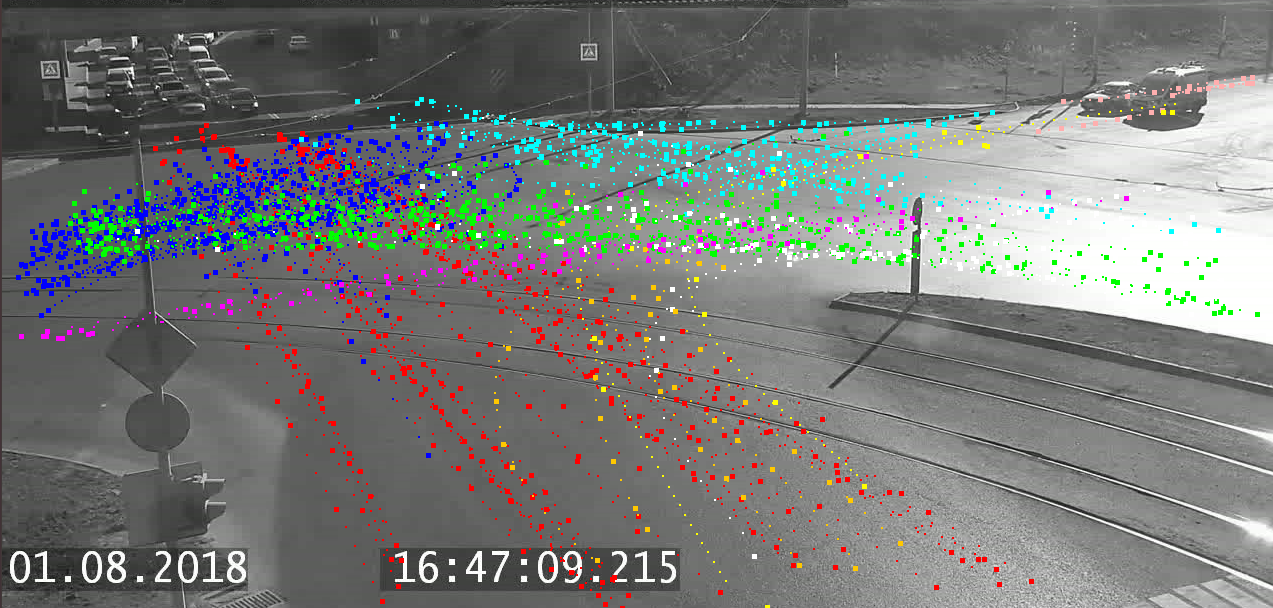
\includegraphics[width=\textwidth]{images/cl-res/2-9cl-015.png}
		\caption{9 clusters, DI = 0.60}
		\label{fig:2-9cl-015}
	\end{subfigure}
	\caption{Clustering results for static $\bm{\varepsilon}$, $coeff_\varepsilon = 0.15$ ($2.txt$)}
	\label{fig:clust-res-2-015}
\end{figure}